% suivi.tex
% 
% author : abisutti
% created : Mon, 19 Oct 2015 13:48:21 +0200
% modified : Mon, 19 Oct 2015 13:48:21 +0200



\documentclass{beamer}

\usepackage[T1]{fontenc}
\usepackage[utf8]{inputenc}
\usepackage[francais]{babel}
\usepackage{array}
\usepackage{tabularx}
\usepackage{multirow}
\usepackage{textcomp}
\usepackage{xstring}
\usepackage{hyperref}

%%% MACRO %%%


% FIXME Prendre en compte les majuscule déjà présente
\makeatletter
\@ifpackageloaded{xstring}{
	\newcommand\smallcaps[1]{\StrLeft{#1}{1}\scriptsize\uppercase{\StrGobbleLeft{#1}{1}}\normalsize }
}{
	\newcommand\smallcaps[1]{\textsc{#1}}
}
\makeatother



%===============================================================================
% Définit un type de puce pour une liste. Si le pakage "pifont" est chargé, il 
% est utilisé, sinon on met un tiret.
\makeatletter
\@ifpackageloaded{pifont}{
	\newcommand\goodItemArrow[0]{\ding{226}}
}{
	\newcommand\goodItemArrow[0]{-}
}
\makeatother



%===============================================================================
% Item de liste avec spécification de la puce et paramètre écrit en gras.
\newcommand\functionality[1]{
	\item[\goodItemArrow] \textbf{#1}\\
}



%===============================================================================
% Commande \Euro indépendante des paquets chargés 
\makeatletter
\@ifpackageloaded{eurosym}{
	\newcommand\Euro[0]{\euro{}}
}{
	\@ifpackageloaded{textcomp}{
		\newcommand\Euro[0]{\texteuro}
	}{
		\newcommand\Euro[0]{Euro}
	}
}
\makeatother



%===============================================================================
% Accès à des variables dans le document. 
%\makeatletter
%\let\titleName\@title
%\let\subtitleName\@subtitle
%\let\authorName\@author
%\makeatother



% Titre de la section courante (que dans beamer)
%\secname 
% Titre de la sous-section courante (que dans beamer)
%\subsecname





\title[R\'eunion de suivi]{Surfaces de r\'evolution discrètes}
\subtitle{R\'eunion de suivi}
\author[]{Zied \smallcaps{Ben} \smallcaps{Othmane} \\ Thomas \smallcaps{Benoist}
	\\ Adrien \smallcaps{Bisutti} \\ Lydie \smallcaps{Richaume}}
\institute{Universit\'e de Poitiers}
\date{3 décembre 2015}

\usetheme{Madrid}
\usecolortheme{sidebartab}
\usefonttheme{professionalfonts}



%%% MACRO %%%


% Vide la barre de navigation
\setbeamertemplate{navigation symbols}{}

%%% DOCUMENT %%%

\begin{document}


%===============================================================================
%	TITRE
%===============================================================================


\begin{frame}
	\titlepage
	
\includegraphics[width=2cm]{../Images/logo-Xlim.png}
	\hfill
	
\includegraphics[width=2cm]{../Images/logo_univ_poitiers.png}
\end{frame}



%===============================================================================
%	INTRODUCTION
%===============================================================================

\section{Introduction}


% --- Équipe -------------------------------------------------------------------
	\subsection{Collaborateurs et clients}
	\begin{frame}{\subsecname}
		\begin{itemize}
			\item Clients~:
				\begin{itemize}
					\item \'Eric \smallcaps{Andres} (Professeur et ancien
						directeur de d\'epartement XLIM-SIC)
					\item Gaëlle \smallcaps{Largeteau}-\smallcaps{Skapin}
						(Maitre de Conf\'erence, G\'eom\'etrie~discr\`ete)
				\end{itemize}
			\item Exemple d'utilisateur final~:
				\begin{itemize}
					\item Aur\'elie \smallcaps{Mourier} (Artiste)
				\end{itemize}
			\item Encadrant p\'edagogique~: 
				\begin{itemize}
					\item Philippe \smallcaps{Meseure} (Professeur, Informatique
						graphique)
				\end{itemize}
		\end{itemize}
	\end{frame}


% --- Contexte -----------------------------------------------------------------
	\subsection{Contexte}
	\begin{frame}{\subsecname}
		\begin{itemize}
			\item Nouvel algorithme conçu par \'Eric \smallcaps{Andres} et
				Gaëlle \smallcaps{Largeteau}-\smallcaps{Skapin} pour mod\'eliser
				des surfaces de r\'evolution discrètes.
			\item Visualisation des r\'esultats avec Mathematica
		\end{itemize}
		\begin{figure}
			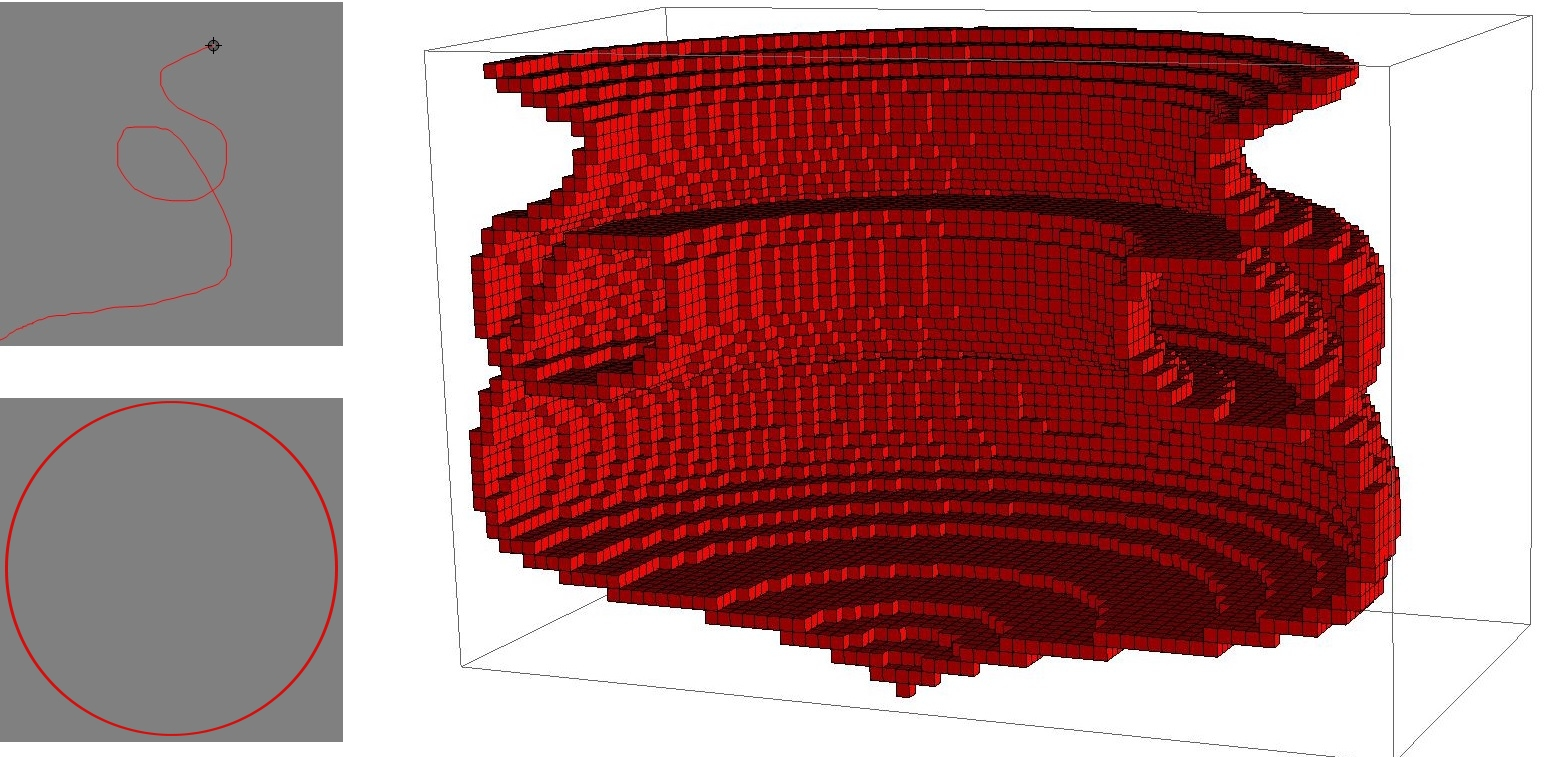
\includegraphics[height=3.8cm]{../Images/revolution2.jpg}
		\end{figure}
		\begin{itemize}
			\item Besoin d'un outil utilisable partout et par tous
		\end{itemize}
	\end{frame}
	


%===============================================================================
%	ORGANISATION
%===============================================================================

\section{Organisation de l'\'equipe}


% --- Roles --------------------------------------------------------------------
	 \subsection{Les r\^oles}
	 \begin{frame}{\subsecname}
		\begin{itemize}
			\item Composition de l'\'equipe~:
				\begin{itemize}
					\item Thomas \smallcaps{Benoist} - Chef de projet
					\item Zied \smallcaps{Ben} \smallcaps{Othmane} - Responsable
						qualit\'e
					\item Adrien \smallcaps{Bisutti} - Responsable des risques
					\item Lydie \smallcaps{Richaume} - Responsable des t\^aches
				\end{itemize}
		\end{itemize}
	\end{frame}



%===============================================================================
%	DEROULEMENT
%===============================================================================

\section{Planification}


% --- Taches -------------------------------------------------------------------
	\subsection{T\^aches}
	\begin{frame}{\subsecname}
		\begin{center}
		{\renewcommand{\arraystretch}{1.3}
		\begin{tabularx}{11cm}{|>{\hfill}X<{\hspace*{\fill}}|X<{\centering}|}
			\hline
			\multicolumn{2}{|c|}{1 - Documentation, test et aide utilisateur}\\
			\hline
			\multicolumn{2}{|c|}{2 - Conception}\\
			\hline
			6 - Noyau fonctionnel & 10 - Interface minimale\\
			\hline
			17 - Ajout de fonctionnalités & \multirow{3}*{14, 22, 32 - 
			Am\'elioration IHM}\\
			\cline{1-1}
			25 - M\'eridienne \`a main levée & \\%Am\'elioration IHM\\
			\cline{1-1}
			29 - Gestion des donn\'ees & \\%Am\'elioration IHM\\
			\hline
			\multicolumn{2}{|c|}{36 - Ajout courbe utilisateur}\\
			\hline
			\multicolumn{2}{|c|}{37 - R\'edaction rapport technique}\\
			\hline
		\end{tabularx}}
		\end{center}
	\end{frame}


% --- Pert ---------------------------------------------------------------------
	\subsection{Diagramme de Pert} 
	% FIXME numéroté les tâches pour pouvoir utilisé cette numérotation
	\begin{frame}{Pert}
		\begin{figure}
			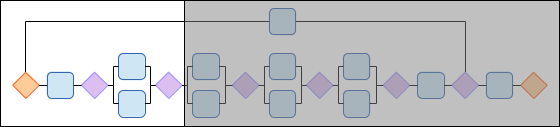
\includegraphics[width=6cm]
				{../Lancement/ImagesLancement/miniature1.png}
		\end{figure}\begin{figure}
			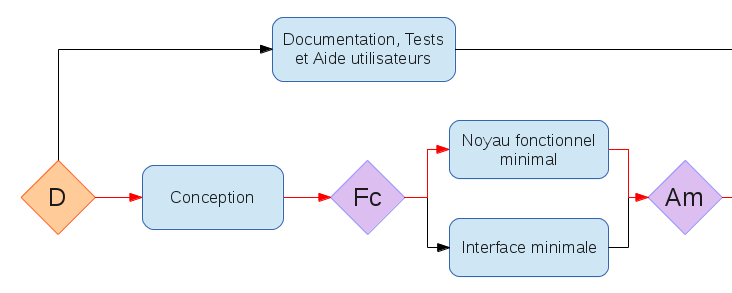
\includegraphics[width=11cm]
				{../Lancement/ImagesLancement/pert_part_1.png}
		\end{figure}
		\footnotesize{D~: D\'epart (30/10) \hfill Am~: Appli. minimale (24/12)\\
			\hfill Fc~: Fin conception (16/12) \hspace*{\fill}}
	\end{frame}

	\begin{frame}{Pert}
		\begin{figure}
			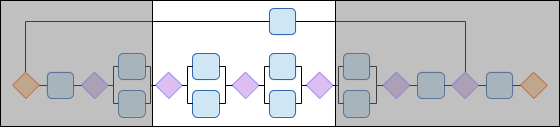
\includegraphics[width=6cm]
				{../Lancement/ImagesLancement/miniature2.png}
		\end{figure}
		\begin{figure}
			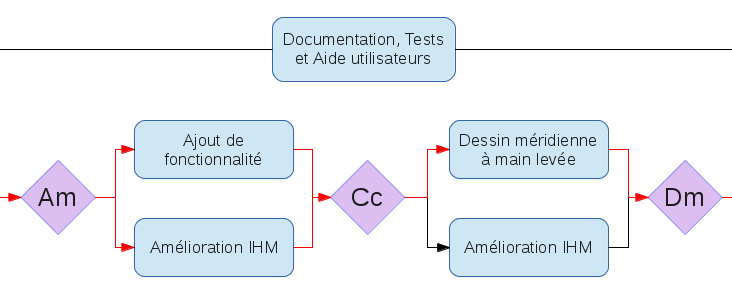
\includegraphics[width=11cm]
				{../Lancement/ImagesLancement/pert_part_2.png}
		\end{figure}
		\footnotesize{Am~: Appli. minimale (24/12) \hfill Dm~: Dessin main 
			lev\'ee (28/01)\\
			\hfill Cc~: Choix des courbes (20/01) \hspace*{\fill}}
	\end{frame}

	\begin{frame}{Pert}
		\begin{figure}
			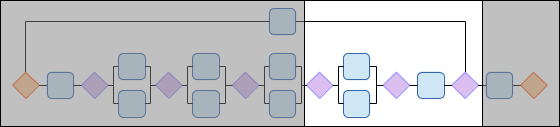
\includegraphics[width=6cm]
				{../Lancement/ImagesLancement/miniature3.png}
		\end{figure}
		\begin{figure}
			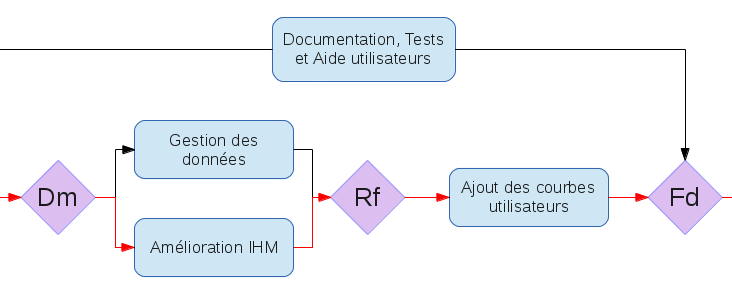
\includegraphics[width=11cm]
				{../Lancement/ImagesLancement/pert_part_3.png}
		\end{figure}
		\footnotesize{Dm~: Dessin main lev\'ee (28/01) \hfill Fd~: Fin 
			d\'eveloppement (02/03)\\
			\hfill Rf~: Rentrer formule (19/02)\hspace*{\fill}}
	\end{frame}

	\begin{frame}{Pert}
		\begin{figure}
			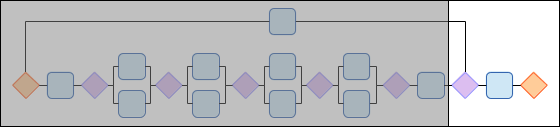
\includegraphics[width=6cm]
				{../Lancement/ImagesLancement/miniature4.png}
		\end{figure}
		\begin{figure}
			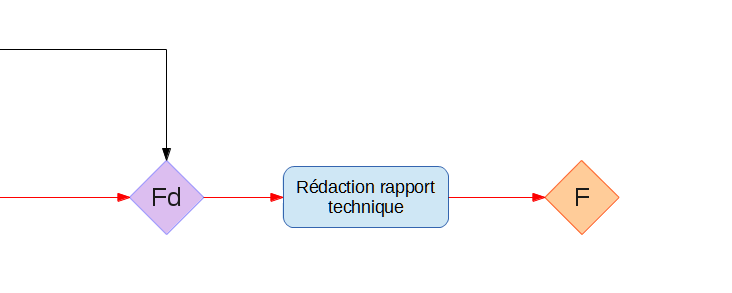
\includegraphics[width=11cm]
				{../Lancement/ImagesLancement/pert_part_4.png}
		\end{figure}
		\footnotesize{Fd~: Fin d\'eveloppement (02/03) \hfill F~: Fin (17/03)\\
			[0.48cm]}
	\end{frame}
	

% --- Gantt --------------------------------------------------------------------
	\subsection{Diagramme de Gantt}
	\begin{frame}{Gantt}
		\begin{center}
			\href{run:Gantt_ProjetDiscretConception.gif}{Ouvrir le Gantt}
		\end{center}
	\end{frame}

% --- Avancement ---------------------------------------------------------------
	\subsection{Avancement réalisé}
	\begin{frame}{\subsecname}
		\begin{figure}
			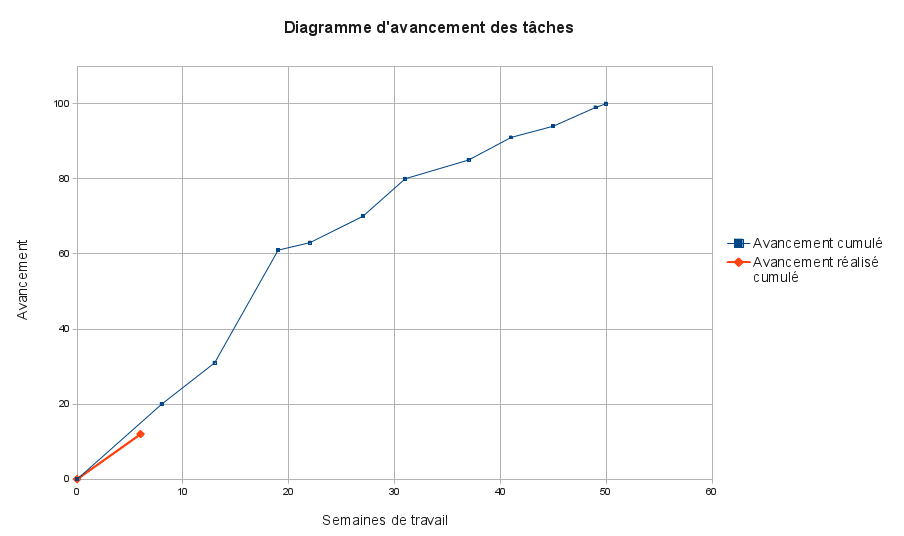
\includegraphics[width=12cm]{Avancement.png}
				% FIXME bien régler les points et faire apparaitre le livrables
		\end{figure}
	\end{frame}


% --- Livrables ----------------------------------------------------------------
	\subsection{Livrables}
	\begin{frame}{\subsecname}
		\begin{center}
%		{\renewcommand{\arraystretch}{1.2}
		\begin{tabular}{|c|m{3cm}|c|c|c|} % FIXME relié les livrables au tâches
			\hline
			\textbf{\No} & \textbf{Livrable} & \textbf{T\^aches}
			& \textbf{Date pr\'evue} & \textbf{Date effective}\\
			\hline
			1 & R\'esultat de l'algorithme et interface & 2, 6, 10 & 23/12 
			& ---\\
			\hline
			2 & Application\break minimale & 14, 17 & 21/01 & ---\\
			\hline
			3 & Courbes avec paramètres modifiables et trac\'e \`a main\break
			lev\'ee& 22, 25 & 29/01 & ---\\
			\hline
			4 & \'Equations et\break export & 29, 32 & 19/02 & ---\\
			\hline
			5 & Application finale et documentation & 36 & 02/03 & ---\\
			\hline
		\end{tabular}%}
		\end{center}
%		Types de livrables~:
%		\begin{itemize}
%			\item Version logicielle~: tous
%			\item Documentation utilisateur~: tous
%			\item Documentation technique~: 1 et 5
%		\end{itemize}
	\end{frame}


%	\begin{frame}{Prochain livrable}
%		\begin{itemize}
%			\item R\'esultat de l'algorithme et interface
%				\begin{itemize}
%					\item 
%					\item 
%				\end{itemize}
%		\end{itemize}
%	\end{frame}


%===============================================================================
%	RISQUES
%===============================================================================

\section{\'Evolution des risques}

	\begin{frame}{\secname}
		\begin{itemize}
			\item Non ad\'equation d'un outil prévu, matériel ou logiciel
		\end{itemize}
		\begin{figure}
			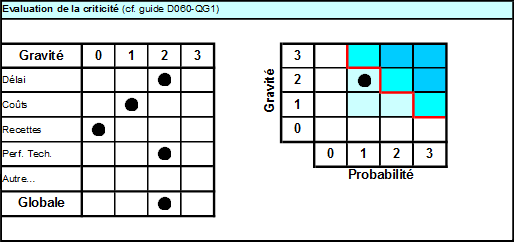
\includegraphics[width=8cm]{risque_outil.png}
		\end{figure}
		\begin{center}
			\begin{tabular}{|c|c|c|c|}
				\hline
				Niveau & Gravit\'e & Probabilit\'e & Criticit\'e \\
				\hline
				0 & Aucune & < 1\% & \multirow{2}*{Non critique}\\
				\cline{1-3}
				1 & Faible (marges) & de 1\% à 5\% & \\
				\hline
				2 & Significative & de 5\% à 20 \% & \multirow{2}*{Critique}\\
				\cline{1-3}
				3 & Danger & > 20\% & \\
				\hline
			\end{tabular}
		\end{center}
	\end{frame}


	\begin{frame}{\secname}
		\begin{itemize}
			\item Nouveau(x) client(s)
		\end{itemize}
		\begin{figure}
			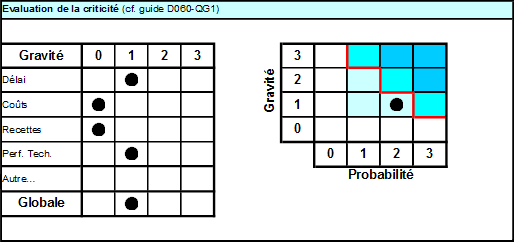
\includegraphics[width=8cm]{risque_nouveau_client.png}
		\end{figure}
		\begin{center}
			\begin{tabular}{|c|c|c|c|}
				\hline
				Niveau & Gravit\'e & Probabilit\'e & Criticit\'e \\
				\hline
				0 & Aucune & < 1\% & \multirow{2}*{Non critique}\\
				\cline{1-3}
				1 & Faible (marges) & de 1\% à 5\% & \\
				\hline
				2 & Significative & de 5\% à 20 \% & \multirow{2}*{Critique}\\
				\cline{1-3}
				3 & Danger & > 20\% & \\
				\hline
			\end{tabular}
		\end{center}
	\end{frame}



%===============================================================================
%	PAQL
%===============================================================================

\section{Plan qualit\'e logiciel}
	\begin{frame}{\secname}
		\begin{columns}
			\begin{column}{8cm}
				\begin{figure}
					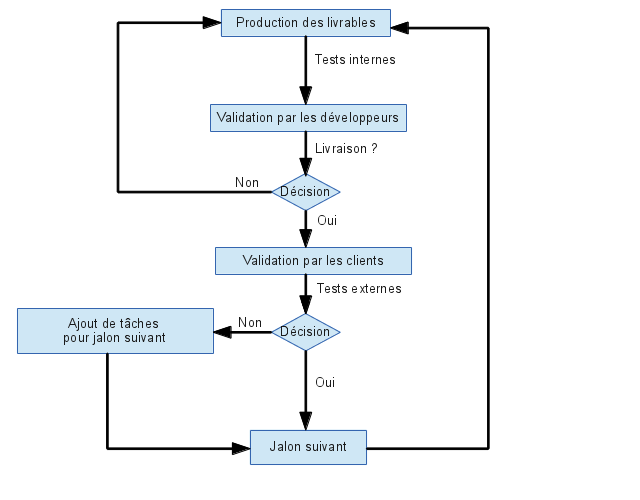
\includegraphics[width=8cm]{PAQL.png}
				\end{figure}
			\end{column}
			\begin{column}{4cm}
				Validation par les clients à chaque jalon.
			\end{column}
		\end{columns}
	\end{frame}



%===============================================================================
%	COUTS
%===============================================================================

\section{Diagramme des coûts}

\begin{frame}{\secname}
	\begin{figure}
		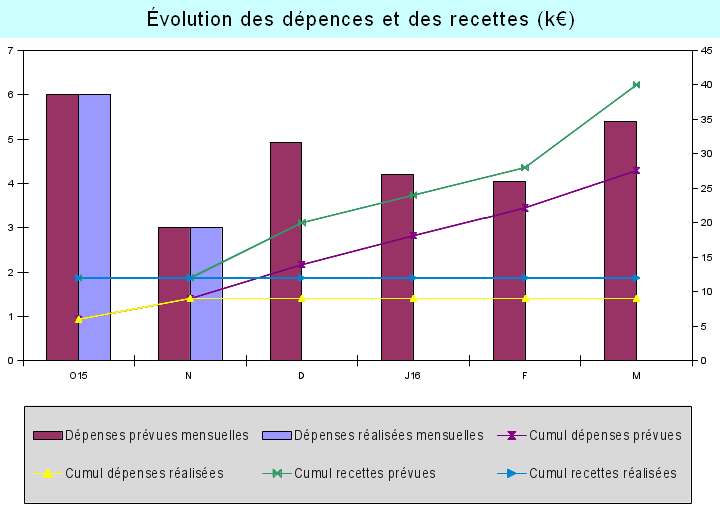
\includegraphics[height=7.5cm]{Cout.png}
		% XXX voir ce que ça donne en semaine
	\end{figure}
\end{frame}



%===============================================================================
%	CONCLUSION
%===============================================================================

\section{À venir}

\begin{frame}{\secname}
	\begin{itemize}
		\item Organiser une réunion avec les nouveaux clients
	\end{itemize}
	\begin{itemize}
		\item Chercher des solveur d'équation
	\end{itemize}
	\begin{itemize}
		\item Terminer la conception 
	\end{itemize}
\end{frame}



\end{document}


